
\documentclass[a4paper, 12pt]{article}
\usepackage[top=3cm, bottom=3cm, left = 2cm, right = 2cm]{geometry} 
\geometry{a4paper} 
\usepackage[utf8]{inputenc}
\usepackage{textcomp}
\usepackage{graphicx} 
\usepackage{amsmath,amssymb}  
\usepackage{bm}  
\usepackage[pdftex,bookmarks,colorlinks,breaklinks]{hyperref}  
\hypersetup{linkcolor=black,citecolor=black,filecolor=black,urlcolor=black} % black links, for printed output
\usepackage{memhfixc} 
\usepackage{pdfsync}  
\usepackage{fancyhdr}
\usepackage{enumitem}
\usepackage{cite}
\usepackage{txfonts}
\usepackage{setspace}
\usepackage{siunitx}
\usepackage{lipsum}
\usepackage{natbib}
\usepackage{eucal}
\usepackage{physics}
\usepackage{color,soul}
\usepackage{subfig}
\usepackage{cancel}
\usepackage[autostyle]{csquotes}
\pagestyle{fancy}
\newcommand{\tn}[1]{\textnormal{#1}}
\graphicspath{{./images}}
\doublespacing

\title{Utrecht University \\
        \large Gravitational waves and observations\\}
\author{Yamamoto Sho}


%\date{}
\begin{document}
\maketitle
\tableofcontents

\section{sonic of Landau-Lifschitz Formalism of EFE}%
  \label{sec:Speedrunning through Landau-Lifschitz Formalism of EFE}
 Define the metric density (which later referred as gothic) as \(
 \mathfrak{g}^{\mu \nu} = \sqrt{-g} g^{\mu \nu}  
 \) and \(
 \mathfrak{g}_{\mu \nu} = \frac{1}{\sqrt{-g}} g_{\mu \nu}  
 \), and of course the kronecker relation \( \mathfrak{g}^{\nu \alpha}
 \mathfrak{g}_{\mu \nu} = \delta_{\mu}^{\alpha} \)
 
 Next, if we chug this whole thing in EFE and make use of these properties,
 one should obtain the the EFE in gothic formalism, 
 \textbf{\textit{Note that:}} this a very important formula, 
  with the kronecker relation, we can partial the whole relation and get, 
  \begin{align}
    \label{partial gothic metric}
    \mathfrak{g}_{\mu \nu} \partial_{\rho}^{} \mathfrak{g}^{\mu \alpha}
    + \mathfrak{g}^{\mu \alpha} \partial_{\rho}^{} \mathfrak{g}_{\mu \nu}
    = 0 
  \end{align}
  Then contract with \( \mathfrak{g}_{\alpha \beta}
   \) and the kronecker relation once again to obtain, 
    \begin{align}
      \label{partial gmet conversion}
      \partial_{\rho}^{} \mathfrak{g}_{\beta \nu} &= -
      \mathfrak{g}_{\alpha \beta} \mathfrak{g}_{\mu \nu}
      \partial_{\rho}^{} \mathfrak{g}^{\mu \alpha}
    \end{align}

  \textbf{\textit{Note 2 that:}} It is also beneficial to obtain the
  relation of gothic versus metric, this can be achieved by, 
  \begin{align}
    \label{getting gothic metric}
    0 = \partial_{\mu}^{} (g_{\alpha \beta} g^{\alpha \beta} ) =
    \partial_{\mu}^{} \bigg( g_{\alpha \beta}
    \frac{\mathfrak{g}^{\alpha \beta}}{\sqrt{-g}}  \bigg) 
  \end{align}
  After some manipulation, we can then get the important conversion
  relation, 
  \begin{align}
    \label{conversion metric and gothic}
    g^{\alpha \beta} \partial_{\mu}^{} g_{\alpha \beta} &=
    \mathfrak{g}^{\alpha \beta} \partial_{\mu}^{}
    \mathfrak{g}_{\alpha \beta} 
  \end{align}

  \textbf{\textit{Note 3 that:}} At last, we consider a mixed indices
  contraction, 
  \begin{align}
    \label{mixed contraction}
    0 = g_{\beta \gamma} \partial_{\mu}^{}( \mathfrak{g}^{\alpha \beta}
    g_{\alpha \rho}  ) \implies 0 = -
    \frac{1}{2} g^{\alpha \beta} g_{\gamma \rho}
    \partial_{\mu}^{} g_{\alpha \beta} + \partial_{\mu}^{}
    g_{\gamma \rho} + g_{\alpha \rho} \mathfrak{g}_{\beta \gamma}
    \partial_{\mu}^{} \mathfrak{g}^{\alpha \beta}
  \end{align}
  where in the second expression we have used conversions between metric and
  gothics. 

  Packing everything up, we get the \enquote{ultimate} relation, 
  \begin{align}
    \label{ultimate conversion}
    \partial_{\mu}^{} g_{\gamma \rho} = - \sqrt{-g}
    \mathfrak{g}_{\alpha \rho} \mathfrak{g}_{\beta \gamma}
    \partial_{\mu}^{} \mathfrak{g}^{\alpha \beta} + \frac{1}{2} \sqrt{-g}
    \mathfrak{g}_{\alpha \beta} \mathfrak{g}_{\gamma \rho}
    \partial_{\mu}^{} \mathfrak{g}^{\alpha \beta}
  \end{align}

  \subsection{EFE in gothic}%
    \label{sub:EFE in gothic}
    

  With all the relation above, we can churn through it all, which is done in
  tutorial 2, to get the EFE (also the Christoffel symbols before)

\begin{align}
  \label{gothicEFE}
  \mathfrak{g}^{\mu \nu} \partial_{\mu}^{} \partial_{\nu}^{}
  \mathfrak{g}^{\alpha \beta}  &= \frac{16 \pi G}{c^4} (-g) T^{\alpha
  \beta} + \underbrace{\Sigma^{\alpha \beta}[\mathfrak{g}, \partial_{}^{}
  \mathfrak{g}] }_{\textrm{nonlinear terms}}. 
\end{align}

And forget about \( \Sigma^{\alpha \beta}  \), its just nonlinear 9 terms.


We then decompose the gothic as \( \mathfrak{g}^{\mu \nu} = \eta^{\mu \nu}
+ h^{\mu \nu} \), with \( \eta^{\mu \nu} \) the flat gothic metric. 

Next, we impose the harmonic coordinate condition, 
\begin{align}
  \label{harmonic coordinate coordinates}
  \partial_{\mu}^{} h^{\mu \alpha} = 0
\end{align}

Finally get the EFEs in  a different form 
\begin{align}
  \label{EFE in different form}
  \Box_{\eta} h^{\alpha \beta} = \frac{16 \pi G}{c^4}
  \tau^{\alpha\beta}, 
\end{align}

where \( \tau^{\alpha \beta} = (-g) T^{\alpha \beta} +
\frac{c^4}{16 \pi G} \mathcal{N}^{\alpha \beta} (h,
\partial_{}^{}h, \partial_{}^{2} h )  \)

\section{energy carried by GWs}%
  \label{sec:energy carried by GWs}
 
 We define GW in the following context (more like a pictorial sense of). 
 \begin{figure}[h!]
 \begin{center}
  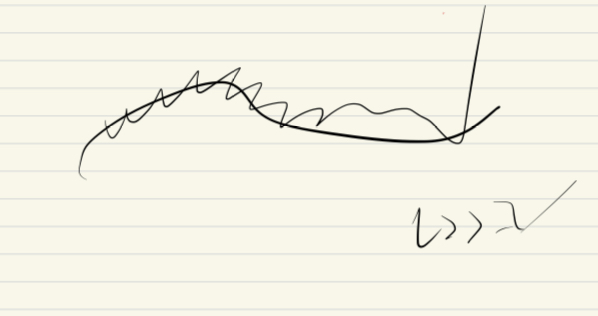
\includegraphics[scale=0.3]{Figures/gravrep.jpeg}
 \end{center}
 \caption{Regardless of the background metric, as long as there is a
   distinct periodicity at some characteristic length, it is a GW signal.}
 \label{fig:gravrep}
 \end{figure}

\textbf{Note: }So the caveat here is that GW is only defined only when there
exists a separation of scales.

Now let 
\begin{align}
  \label{gothic metric expansion}
  \mathfrak{g}^{\mu \nu} = \eta^{\mu \nu}_{(1)} + \epsilon h^{\mu \nu}_{(1)}
  + \epsilon^{2} h^{\mu \nu}^{(2)}.  
\end{align}, note that everything here are gothics but not metric tensors. 

Next we impose the gauge fix \( \Box_{\eta} \eta^{\alpha \beta} = 0
\implies \eta = \mathrm{const.} \)

And we can tackle the EFE by recursive perturbation, which reads for the
first two orders as 
\begin{align}
  \label{perturbation on EFE}
 \begin{cases} 
   \Box_{\eta} h^{\alpha \beta}_{(1)} &= 0  \\
   \Box_{\eta} h^{\alpha \beta}_{(2)} &= \mathcal{N}^{\alpha \beta} [
   h_{(1)}].
 \end{cases} 
\end{align}
The first order corresponds to simply the waves, with purely oscillation.
The second order however corresponds to the second order term, which has
both energy and oscillation perturbation, this is because second order terms
goes like \( \Box^2 h, \) which indeed appears in EFE (\ref{EFE in different
form}). "Explicitly", we can denote these solutions as \( h^{\alpha
\beta}_{(1)} = \hat{h}^{\alpha \beta}
_{(1)}, \textnormal{ and } \hat{h}
^{\alpha\beta}_{(2)} = \hat{h}
^{\alpha \beta}_{(2)}  + \langle h_{(2)}^{\alpha \beta} \rangle \)
and in particular the averaged term indeed does show up in the EM tensor. 

\subsection{Lightning review of \( \langle \cdot \rangle \)
operator}%
  \label{sub:Lightning review of \( \langle \cdot \rangle \) operator}
 \begin{enumerate}
   \item[\cdot] It commutes with \( \Box_{\eta} \)
 \end{enumerate} 
 \( \textnormal{i.e.} [  \Box_{\eta}, \langle \rangle ] = 0   \)
 which implies $ \Box(\langle h_{(1)}^{\alpha \beta} \rangle + \hat{h}
 _{(2)}^{\alpha \beta}) = 0$

 So we naturally obtain 
 \begin{align}
  \label{some}
   \Box(\cancelto{0}{\eta^{\alpha \beta}} + \epsilon
   \cancelto{0}{h_{(1)}^{\alpha \beta}} + \epsilon^2 \langle h^{\alpha
   \beta}_{(2)} \rangle  ) = \epsilon^2 \langle
   \mathcal{N}^{\alpha \beta}_{(2)} \equiv \frac{32 \pi G}{c^4}
   \tau_{\alpha \beta}^{\mathrm{eff, GW}} 
 \end{align}

 \section{Slightly different from linearized gravity}%
  \label{sec:Slightly different from linearized gravity}
  In our previous formalism, GWs source are not corrected to
  "background" at 2nd order. And thus we missed out on the coarse-grain
  effects of GWs. 
  \subsection{ Packaging up the formalism }%
    \label{sub: Packaging up the formalism }
    In order to obtain the energy-momentum tensor contributed by the
    gravitational wave, we can follow the procedure as follows 
    \begin{enumerate}
      \item[\it 1. ]  Assume TT-gauge and implement average over \(
       \mathcal{L} \gg \lambda  \) and use I.B.P. multiple
       throughout the calculation below, 
       \begin{align}
        \label{calc average metric}
         \langle h^{\alpha \beta} \partial_{\alpha}^{}
         \partial_{\beta}^{} h^{\mu \nu} \rangle = \langle
         \partial_{\alpha}^{} ( h^{\alpha \beta
         \partial_{\eta}^{} h^{\mu \nu} } ) - \langle
         (\cancelto{0}{\partial_{\alpha}^{} h^{\alpha
         \beta}})(\partial_{\beta}^{} h^{\mu \nu}) \rangle . 
       \end{align}, the 2nd term is zero due to harmonic gauge.
      \item[\it 2.] From here, we further massage (\ref{calc average
      metric}) via the three tricks below: 
      \begin{align}
        \label{average metric tricks}
        \begin{cases} 
          \partial_{\mu}^{} h^{\alpha \beta} \partial_{\gamma}^{}
          h^{\mu \delta} &= \partial_{\mu}^{} ( h^{\alpha \beta}
          \partial_{\gamma}^{} h^{\mu \delta} ) - h^{\alpha \beta}
          (\partial_{\gamma}^{} \cancelto{0}{\partial_{\mu}^{}
          h^{\mu \delta}}) \\
        \partial_{\mu}^{} h^{\mu \beta} &= 0 \\ 
          \partial_{\alpha}^{} \partial_{}^{\alpha} h_{(1)}^{\mu
          \nu} &= 0
        \end{cases} 
      \end{align}
      1st is simply I.B.P., 2nd is harmonic gauge condition, and 3. is
      ?
      \item[\it 3.] Keep working then one will eventually obtain the
      expression 
      \begin{align}
        \label{GW contribution to energy momentum tensor}
        t_{\mu \nu}^{\mathrm{GW}} &= \langle \frac{c^4}{32 \pi G} \langel
        \partial_{}^{\mu} h_{\alpha \beta}^{(1)} \partial_{}^{\nu}
        h_{(2)}^{\alpha \beta} \rangle 
      \end{align}
    \end{enumerate}

    And here \( t^{00}_{\textnormal{GW}}  \) is defined as the GW energy
    density, which written explicitly as 
    \begin{align}
      \label{GW energy density}
      t_{\mathrm{GW}}^{00} &= \frac{c^2}{32 \pi G} \langle \hat{h}_{ij}
      \hat{h}^{ij} \rangle = \frac{c^2}{16\pi G} \langle
      \dot{h}_{+}^{2} + \dot{h}_{\cross}^{2} \rangle
    \end{align}
The \( c^2 \) is suppressed by \(  \partial_{0}^{} = 1/c \partial_{}^{} \)


The GW power is then defined as, 
\begin{align}
  \label{GW power}
  \frac{\mathrm{d}E_{\mathrm{GW}}}{\mathrm{d}t} &=
  \frac{\mathrm{d}}{\mathrm{d}t} \int_{\nu} \mathrm{d}^{3}x \hspace{0.1cm}
  t_{00}^{\mathrm{GW}} = c \int_{\nu} \mathrm{d}^{3}x 
  \partial_{0}^{} t_{\mathrm{GW}}^{00} 
\end{align}

Next, we can impose conservation law such that \(
\partial_{\mu}^{} t_{\mathrm{GW}}^{\mu \nu} = 0 \), which implies \(
\partial_{0}^{} t_{00}^{\mathrm{GW}} + \partial_{0}^{}
t_{\mathrm{GW}}^{0i} = 0 \), and it implies finally \( \partial_{0}^{}
t_{\mathrm{GW}}^{00} = - \partial_{0}^{} t_{\mathrm{GW}}^{0i}\)

Therefore we perform gauss law on (\ref{GW power}), 
\begin{align}
  \label{gauss law on GW power}
  \frac{\mathrm{d} E_{\mathrm{GW}}}{\mathrm{d}t} &= c \int_{\nu}
  \mathrm{d}^{3}x ( - \partial_{i}^{} t_{\mathrm{GW}}^{0i} ) \\ 
  &= c \int_{S} \mathrm{d}^{2}x (u^i t_{\mathrm{GW}}^{0i})
\end{align}
where \( u^i \) is the unit normal to the surface S.

The pictorial interpretation is as follow 
\begin{figure}[h!]
\begin{center}
  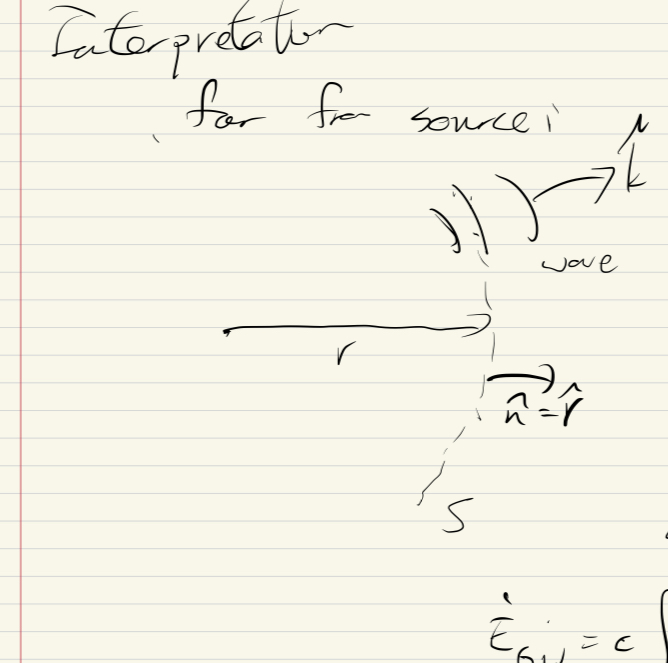
\includegraphics[scale=0.3]{Figures/pictorial_interpretation.jpeg}
\end{center}
\caption{this is the pictorial representation of (\ref{gauss law on GW
  power}).}
\label{fig: pictorial representation on gauss law on GW power}
\end{figure}

So we approximately get \( h_{ij} \approx h_{ij}(t - r/c) \implies
\partial_{i}^{} h(t-r/c) = 1/c \partial_{t}^{} h (t -r/c) = -
\partial_{0}^{}h(t-r/c) \), and in this case \(
t_{\mathrm{GW}}^{0i} = - t_{\mathrm{GW}}^{00} \), and finally arriving at 
\begin{align}
  \label{GW final power expression }
  \dot{E}_{\mathrm{GW}} &= c \int_S \mathrm{d}^{2}\Omega r^2
  t_{\mathrm{GW}}^{00} = \underbrace{\frac{c^3}{16 \pi
  G}}_{\textrm{crazy huge term } c^3/G \sim 
  10^{35}\mathrm{kg/s}} r^2 \int
  \mathrm{d}^{2}\Omega \langle \dot{h}_{+}^{2} +
  \dot{h}_{\cross}^{2} \rangle
\end{align}

And the flux can be simply defined as 
\begin{align}
  \label{Flux GW}
  F_{\mathrm{GW}} = \frac{c^3}{16 \pi G} \langle \dot{h}_{+}^{2} +
  \dot{h}_{\cross}^{2} \rangle \iff \textnormal{ GW also carry Energy Momentum }
\end{align}


\newpage

\begin{figure}[h!]
\begin{center}
  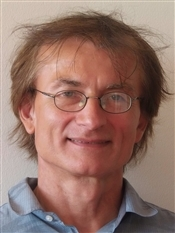
\includegraphics[scale=2]{Figures/thomas.jpeg}
\end{center}
\caption{Here lies a picture of thomas.}
\label{fig:thomas boy}
\end{figure}

\newpage


\section{BBH GWs}%
  \label{sec:BBH GWs}
 In this section, we solely look into all the GWs possibly produced by
 studying a BBH scenario. 
 \subsection{Level-Matching of asymptotic expansion}%
  \label{sec:Level-Matching of asymptotic expansion}
 
 \begin{figure}[h!]
 \begin{center}
  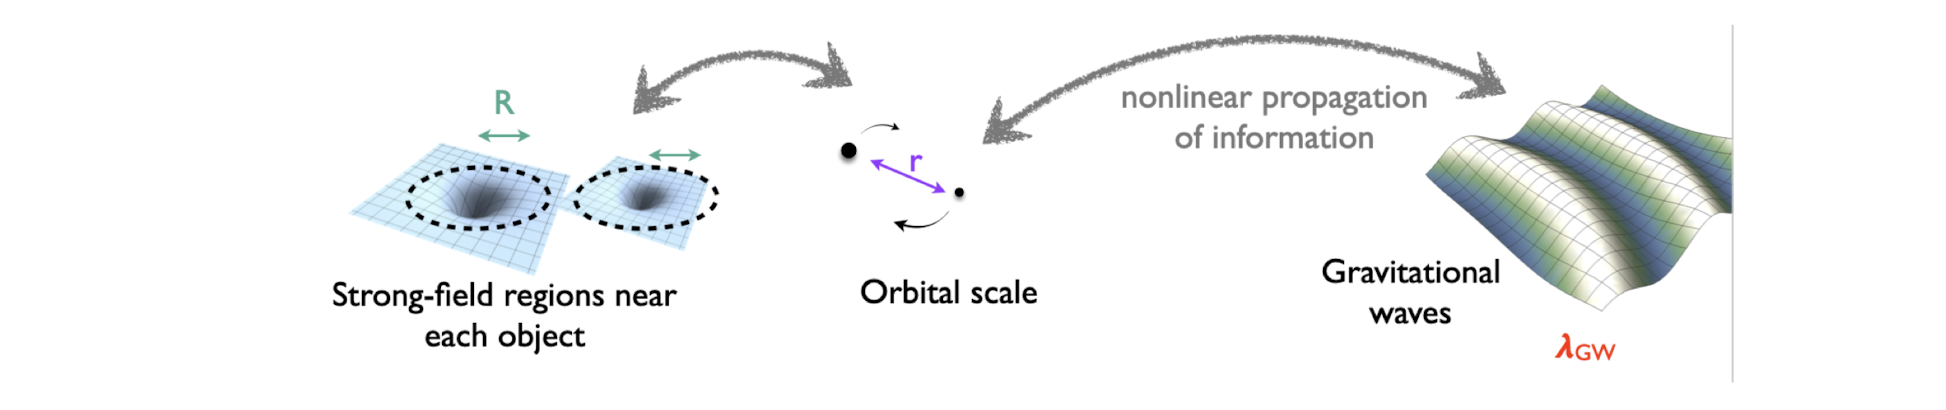
\includegraphics[scale=0.3]{Figures/levelmatching.png}
 \end{center}
 \caption{Schematic information flow from a binary source to GWs. Different
   descriptions are required in different patches of the
   spacetime.}
 \label{fig:Schematic of levelmatching}
 \end{figure}

 The upshot of this figure is that, spacetime behaves very different
 on different scales, and this is reflected in during the matched asymptotic
 expansion. 

\subsubsection{Simple example of asymptotic expansion}%
  \label{sub:Simple example of asymptotic expansion}
 We aim to solve the ODE: 
 \begin{align}
  \label{ODE}
   \epsilon y^{(1)}(x) + y^{(1)}(x) + 3y(x) = 0, \hspace{0.5cm} \epsilon
   \ll 1
 \end{align}, with b.c. \( y(0) = 0, \hspace{0.1cm} y(1) = 1 \).
 
 Now we approximate in the far zone via 
 \begin{align}
  \label{far zone approx}
   y = y_0(x) + \epsilon y_1(x) + \mathcal{O}(\epsilon^2)
 \end{align}

 Then we solve the ODE by neglecting \( \mcal{O}(\epsilon^2) \) to get 
 \begin{align}
  \label{far zone expansion}
   \epsilon y^{\prime \prime}_{0} + y_0^{\prime} + \epsilon
   y_1^{\prime} + 3 y_0 + 3 \epsilon y_1 = \mcal{O}(\epsilon^2)
 \end{align}

 by collecting the \( \epsilon \) in terms of their orders we get 
 \begin{align}
  \label{1st case packaged}
  \begin{cases} 
    &\mcal{O}(\epsilon^0): y_{0}^{\prime} + 3y = 0 \to y_0 = c_1 e^{-3x}
    \\ 
    &\mcal{O}(\epsilon^1): y_{1}^{\prime} + 3 y_1 = -
    y_{0}^{\prime \prime} \to y_1 = c_2 e^{-3x} - 9 c_1 x e^{-3x}  \\ 
    &\mcal{O}(\epsilon^2): \cdots
  \end{cases}
 \end{align}

 and of course we get the coefficients by imposing b.c. and we get \( c_1
 = e^{3}, \hspace{0.1cm} c_2 = 9 e^3 \)
Then we plug these back into (1) to get the near zero-zone approx of y 
\begin{align}
  \label{final far zone expansion}
  y =  e^{3 - 3x} + 9 \epsilon e^{3-3x} (1 - x) +
  \mcal{O}(\epsilon^2)  
\end{align}

\textbf{Comments: }

\begin{enumerate}
  \item[\cdot] Note that this expression fails at far zone, but fails at
  \( x \to 0 \) fails. 
\end{enumerate}

Now, we aim for the zero-zone expression, 

\begin{align}
  \label{new variable}
  X &= \frac{X}{\epsilon} = \mcal{O}(1) \hspace{0.5cm}
  \mathrm{for} \hspace{0.1cm} x = \mcal{O}(t)
\end{align}
The interpretation for this variable is that, it \enquote{streches} the region of small x. 

Now consider the limit \( \epsilon \to 0 \) at fixed X. 
We will obtain the ansatz, 
\begin{align}
  \label{inner field expansion}
  y^{\mathrm{Inner}} = y_0(x) + \epsilon y_{1}(x) +
  \mcal{O}(\epsilon^2)  
\end{align}, with the  derivative swapped as 
\begin{align}
  \label{yep}
  \frac{\mathrm{d}}{\mathrm{d}x} =
\frac{\mathrm{d}X}{\mathrm{d}x} \frac{\mathrm{d}}{\mathrm{d}x} =
\frac{1}{\epsilon} \frac{\mathrm{d}}{\mathrm{d}x} 
\end{align}

The ODE now reads: 
\begin{align}
  \label{reads}
  \frac{1}{\epsilon} Y_{0}^{\prime \prime} + Y_{1}^{\prime \prime} +
  \frac{1}{\epsilon} y_{0}^{\prime} + y_{1}^{\prime} + 3 y_{0} =
  \mcal{O}(\epsilon)
\end{align}

And if we keep track of the order of \( \mcal{O}(\epsilon) \) we further get, 


\begin{align}
  \label{zero zone approx}
  \begin{cases} 
    &\mcal{O}(\epsilon^{-1}):  y_{0}^{\prime \prime} +
    y_{0}^{\prime} = 0 \\ 
    &\mcal{O}(1): y_{1}^{\prime \prime} + y_{1}^{\prime} = - 3 y_{0}
  \end{cases}
\end{align}

The ansatz is thus, 
\begin{align}
  \label{zero-zone ansatz}
  y_{0} = c_1 e^{-x} + c_2  
\end{align}
And imposing b.c., we further get \( y_0(0) = 0 \to c_2 = -c_1 \)
And finally 

\begin{align}
  \label{final outer inner}
  \begin{cases} 
    &y^{\mathrm{outer}} = e^{3-3x} + \epsilon_1 9 e^{3-3x} (1-x) +
    \mcal{O}(\epsilon^2) \\ 
    &y_{\mathrm{inner}} = c_1 (e^{-x} - 1 ) + B_1 c (x-1) +
    e^{2x}(\cdots) 
  \end{cases}
\end{align}

\textbf{Comment: } Please notice the \( \epsilon \) dependence in the
equation, this means that this approximation does depend on one extra
parameter now, kinda magical to say.
 
We can plot these as 

\begin{figure}[h!]
  \centering
    \subfloat[]{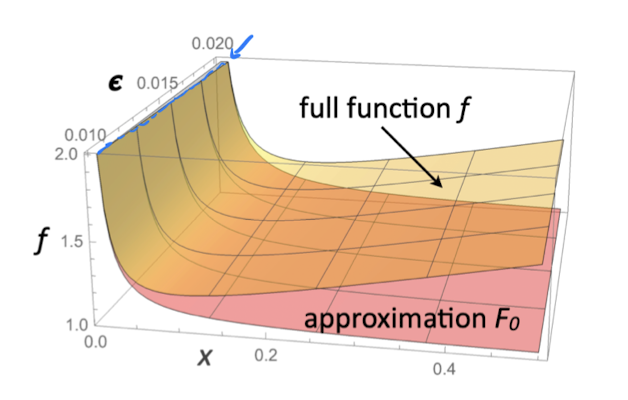
\includegraphics[scale=0.4]{Figures/asymp2.png}\label{fig:leading-order inner}}
    \subfloat[]{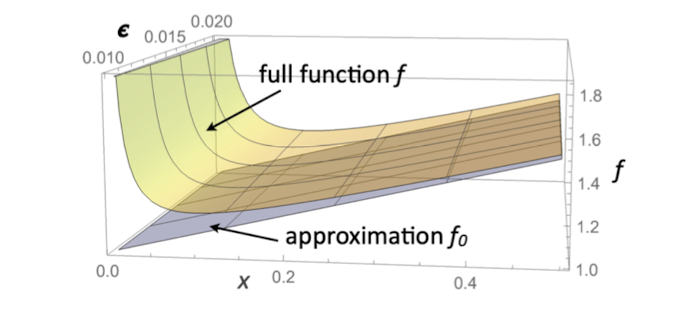
\includegraphics[scale=0.4]{Figures/asymp.png}\label{fig:leading-order outer}}
     \caption{(a) The leading order outer approximation, (b) the leading order inner approximation}
\end{figure}

One can easily see that the extra \( \epsilon \) degrees of freedom when doing the approximation.

\subsection{intermediate regime}%
  \label{sub:intermediate regime}
  Now we can see that the approximation fails at both ends, and the natural
  question to ask is whether there exists an approximation such that we
  can speak of the overlapping domain. And this section talks about such
  approach.

  So in the intermediate regime of x small, and X large, we expect both expansions
  are valid. We can formalize this by introducing a function \(
  \eta(\epsilon)   \) with \( \epsilon \ll \eta(\epsilon) \ll 1 \), and note
  that this naturally has to be a range, e.g. \( \epsilon^{1/2} \ll \eta
  \ll \epsilon \).

  Thus we define in the intermediate domain: 
  \begin{align}
    \label{intermediate domain Xes}
    \begin{cases} 
      x &= \mcal{O}(\eta), \hspace{0.5cm} \textnormal{small as } \epsilon
      \to 0 \\ 
      x &= \mcal{O}(\frac{\eta}{\epsilon}), \hspace{0.5cm}
      \textnormal{large as } \epsilon
      \to 0
    \end{cases}
  \end{align}

  We also introduce a scaled coordinate that is \( \mcal{O}(1) \) in this
  regime: 
  \begin{align}
    \label{intermediate x}
    x_{\eta} &= \frac{x}{\eta}
  \end{align}
  And by imposing the matching condition, as \( \epsilon \to 0 \) \begin{align}
    \label{intermediate matching}
    \lim_{\epsilon \to 0} [ y^{\mathrm{inner}}(x_{\eta}) -
    y^{\mathrm{outer}}(\eta)  ] = 0
  \end{align}

Next, we convert solutions to \( x_{\eta} \). 

The inner solution reads, 
\begin{align}
  \label{converting to inner y}
  y^{\mathrm{inner}}(x_{\eta}) &= C_0 ( e^{-
  \frac{\eta(\epsilon)}{\epsilon}x_{\eta}} - 1  ) + 3 C_0 \eta x_{\eta}
  ( 1 + e^{- \frac{\eta(\epsilon)}{\epsilon} x_{\eta}} ) + \epsilon
  (3 C_0 + C_1) ( e^{- \frac{\eta(\epsilon)}{\epsilon} x_{\eta}} -
  1) + \cdots \\ 
  &\approx -C_0 + 3C_0 \eta x_{\eta} - \epsilon (3 C_0 + C_1) + \mcal{O}(
  e^{- \frac{\eta(\epsilon)}{\epsilon}} ) + \cdots, 
\end{align}
and the outer solution reads, 
\begin{align}
  \label{converting to outer y}
  y^{\mathrm{outer}}(x_{\eta}) &= e^{3 - 3 \eta(\epsilon) x_{\eta}}
  + 9 \epsilon e^{3 - 3 \eta(\epsilon) x_{\eta}} - 9 \epsilon \eta
  x_{\eta} e^{3 - 3 \eta(\epsilon) x_{\eta}} + \cdots \\ 
  &= e^3 - 3 e^3 \eta x_{\eta} + 9 \epsilon e^3 + \mcal{O}(\epsilon
  \eta, \eta^2) + \cdots
\end{align}

And by imposing the criteria of (\ref{intermediate matching}), or
\hl{intuitively, both } (\ref{converting to inner y}) \hl{and
} (\ref{converting to outer y}) are in terms of the new variable \( x_{\eta}
\), thus the comparison is reasonable, and taking the limit \( \epsilon \to
0 \), simply (1) is the only for us to conduct the matching; (2) 
it is technically imposing \( \eta \to 0 \) at the same time.

Now we hunt down the coefficient by matching the \( \mcal{O}(\epsilon) \)
orders. 

\begin{align}
  \label{matching gives}
  \begin{cases} 
    &\mcal{O}(1) \mathrm{ terms:  } \hspace{0.5cm} C_0 = -e^3 \\
    &\mcal{O}(\epsilon) \mathrm{ terms: } \hspace{0.5cm} C_1 = -6e^3
  \end{cases}
\end{align}



\begin{figure}[h!]
\begin{center}
  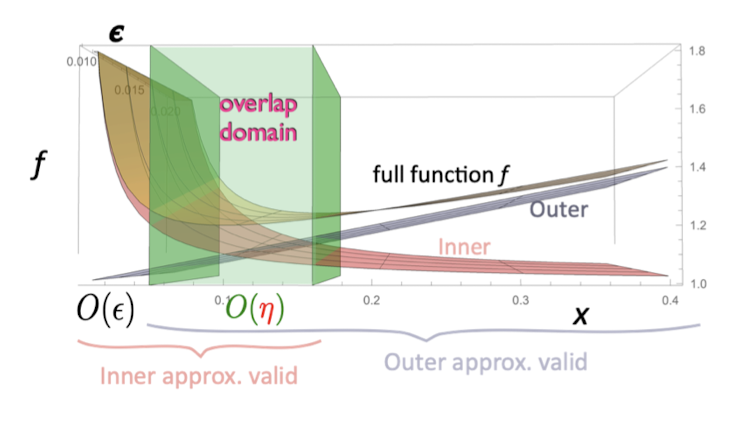
\includegraphics[scale=0.5]{Figures/mixasymp.png}
\end{center}
\caption{shows all the approximation region with the extra \( \eta \)
  parameter space.}
\label{fig:mixasmpy}
\end{figure}

\subsection{Composite expansion and comparisons}%
  \label{sub:Composite expansion and comparisons}
  To obtain the composite solution, we essentially add distinct terms from
  \( y^{\mathrm{inner}}  \) and \( y^{\mathrm{outer}}  \), and then
  subtract the common terms. 
  If we fall back to the previous example then we are trying to add
  (\ref{converting to inner y}) and (\ref{converting to outer y}) and then
  subtracting the double-counting of the common terms, which gives 
  \begin{align}
    \label{composite y}
    y^{\mathrm{composite}} = e^{3}(1 - e^{-\frac{x}{\epsilon}}) +
    e^{3(1-x)} - e^{3} + \cdots = e^{3 - 3x} - e^{3 -
    \frac{x}{\epsilon}} + \cdots    
  \end{align}




\begin{figure}[h!]
\begin{center}
  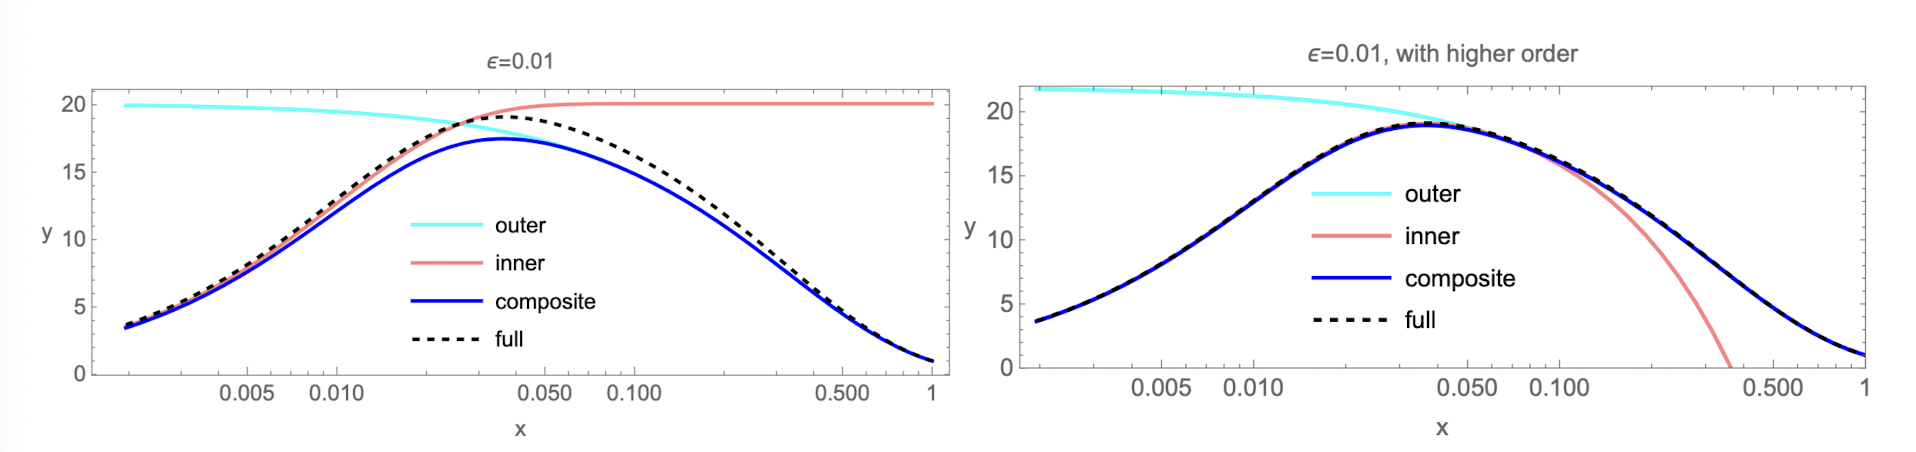
\includegraphics[scale=0.5]{Figures/levelmatched.png}
\end{center}
\caption{shows the plots with different approximation at a given \( \epsilon \)}
\label{fig:levelmatched}
\end{figure}







\textbf{Comment: }
Of course there is the natural question to ask why there is no turning
points within the function, in fact, it may or may not have at the end of
the day, and if we figure so, then we have to do further inner-inner
approximation (or
any combination).



  \section{Post-Newtonian (PN) theory for GWs}%
    \label{sec:Post-Newtonian (PN) theory for GWs}
    In this section we aim to study compact-objects binaries in the
    regime where post-newtonian theory is needed. 

    To start off, it is instructive to ask what is the regime where PN
    approximation is needed. PN approximation is valid for
    \hl{semi-relativistic systems that are graivtationally bound, where
    the typical velocities are } \(  v^2 / c^2 \sim GM / r c^2 \ll 1, \)
    and it is also combined with an approximation in the distant wave
    zone known as the \textit{multipolar post-Minkowski expansion.}
\begin{figure}[h!]
\begin{center}
  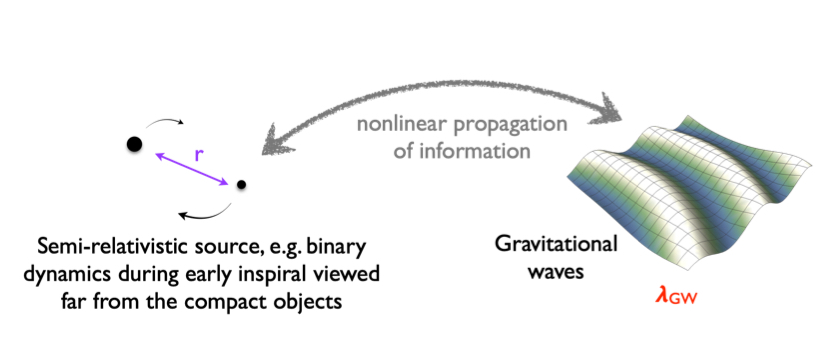
\includegraphics[scale=0.5]{Figures/PNapprox.jpeg}
\end{center}
  \caption{The post-Newtonian (PN) approximation is suitable for describing
  the dynamics and GWs of a point-mass binary system during the early
  inspiral, when the motion is semi-relativistic. THe term 'PN' is often
  loosely used for the entire description, which involves matching
  PN expansion in the regions near the source to a multipolar
  post-Minkowski approximation in adpated to the wavezone at large
  distances from the source.}
\label{fig:PN approximation}
\end{figure}



It is somewhat useful to define the following dimensionless
characteristic parametrs for the binary system, they are: 

\(  \textnormal{mass ratio: } m/M, \hspace{0.5cm} \textnormal{objects' internal
gravity: }GM/rc^2,\\
\hspace{0.5cm} \textnormal{objects'size compared to orbit: } R/r, \hspace{0.5cm}
\textnormal{gravitational interaction potential: } GM/rc^2,
\hspace{0.5cm}\textnormal{velocity: } 
v/c. \)

And the PN limit we are describing are that (i) it is semi-relativistic
\(  v^2 / c^2 \ll 1 \) and weakly gravitating \( GM/rc^2 \ll 1 \) and
gravitationally bound \( ( v^2/c^2 \sim GM/rc^2 ) \). 

\begin{figure}[h!]
\begin{center}
  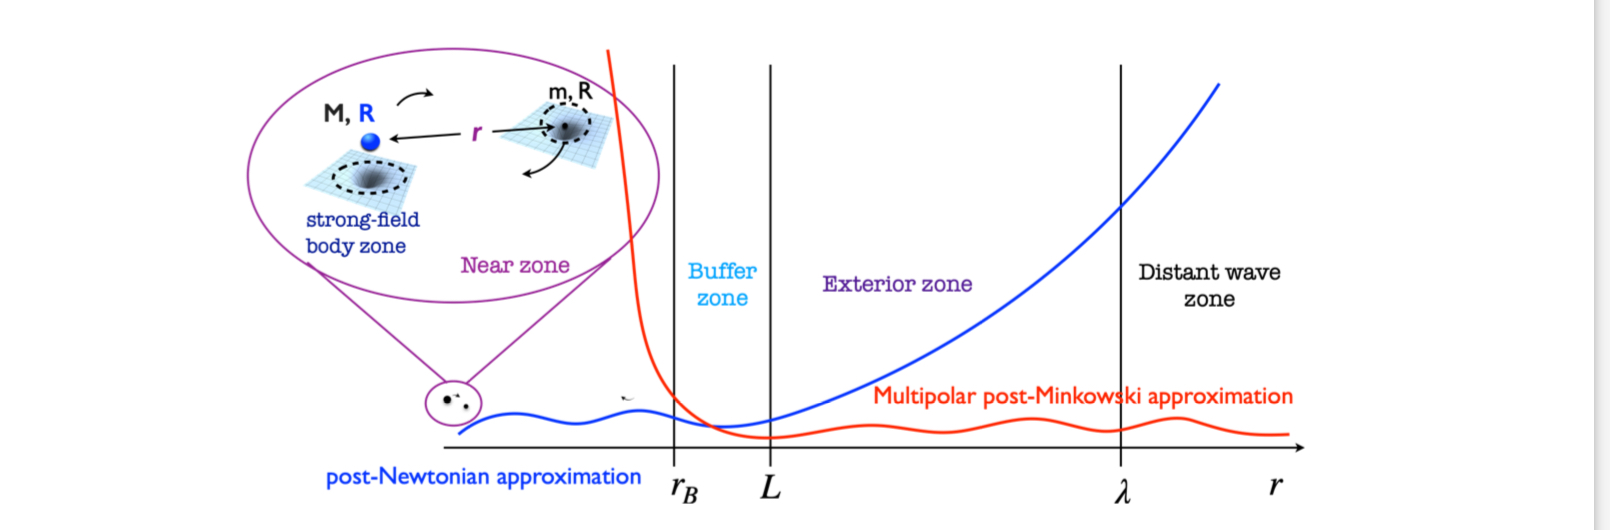
\includegraphics[scale=0.3]{Figures/PNcompare.jpeg}
\end{center}
\caption{Example of the hierachy of scales in the two-body problem and
  the application of the method of matched asymptotic expansion connecting
  a post-Newtonian expansion in the near-zone to the post-Minkowski
  expansion in the wave zone.}
\label{fig:PNcompare}
\end{figure}

\subsection{Commence the PN analysis}%
  \label{sub:Commence the PN analysis}
  Formally, we will use \( 1/c \) as the expansion parameter, and for each
  factor of \( 1/c^2 \) we treat it as 1 PN order. 

  And the matter source behaves like, 
  \begin{align}
    \label{PN EM tensor}
    T^{\alpha \beta} &\sim \textnormal{ Newt. rel. corr., i.e. } T^{00}
    \sim \rho c^2  \\ 
    &\sim c^2 T_{(0)}^{\alpha \beta} + \mcal{O}(c) 
  \end{align}

  And if we put this into the gothic EFE formalism, 
  \begin{align}
    \label{gothic PN}
    \Box h^{\alpha\beta} &=  \frac{16 \pi G}{c^4} [ -g ( c^2
    T_{(0)}^{\alpha \beta} + \mcal{O}(c) ) + \mathcal{N}^{\alpha \beta}  ]
    \\ 
    &\sim \frac{16 \pi G}{c^2} \tau_{(0)}^{\alpha \beta} +
    \mcal{O}(\frac{1}{c^3})
  \end{align}

  The upshot with looking at PN theory in gothic EFE is that the gothich
  EFE becomes a perturbative system in \(  \mcal{O}(1/c) \), i.e. of the
  form \(  \Box h_{(0)}^{\alpha \beta} = 16 \pi G T_{(0)}^{\alpha \beta}
  \cdots \), and you can go up to higher-order as one pleases.
  
  And the solution for the 0-th order via integration (green-function
  is obtained) takes the form, 
  \begin{align}
    \label{0th order PN h}
    h_{(0)}^{\alpha \beta} &= - 4G \int \dd[]{t^{\prime}} 
    \dd[3]{\textbf{x}^{\prime}} \frac{}{} \frac{\tau_{(0)}^{\alpha
    \beta} ( t^{\prime}, \textbf{x}^{\prime} )}{ | \textbf{x} -
    \textbf{x}^{\prime} } \delta ( t^{\prime} - t  +
    \frac{\textbf{x} - \textbf{x}^{\prime}}{c} ) \\ 
    &= - 4G \int_{\mathbb{R}} \dd[3]{\textbf{x}^{\prime}} \underbrace{
    \tau_{(0)}^{\alpha \beta} \frac{( t - \frac{\textbf{x} -
    \textbf{x}^{\prime}}{c}, \textbf{x}^{\prime} )}{ ( \textbf{x}
    - \textbf{x}^{\prime}) } }_{I^{\alpha \beta},
    \textnormal{  quadrupole moment.}}
  \end{align}

And one can see the retardation time appearing in this expression. 


\subsection{Near-zone expansion: }%
  \label{sub:Near-zone expansion: }
  Near-zone, as its name suggests describes the dynamics close the the
  binary where PN limit is adopted, and note that in this regime the
  retardation effects are small and the potentials are nearly
  instantaneous, so the equation of motion reduce to some U-potential.
  and we get something for the quadrupole moment like, 

  \begin{align}
    \label{quadrupole moment}
    I_{nz} \approx \frac{\tau(t, \textbf{x}^{\prime})}{ |
    \textbf{x} - \textbf{x}^{\prime} } + \frac{\dot{\tau}(t,
    \textbf{x}^{\prime})}{| \textbf{x} - \textbf{x}^{\prime} |} ( -
    \frac{| \textbf{x} - \textbf{x}^{\prime}}{ c } ) +
    \frac{1}{2}
    \frac{\ddot{\tau}}{| \textbf{x} - \textbf{x}^{\prime} |} \frac{|
    \textbf{x} - \textbf{x}^{\prime} |^2}{c^2}
  \end{align}

  Now note that the potentials are instantaneous, so we can further do 

  \begin{align}
    \label{h form in near-zone}
    h_{(0)}^{\alpha \beta, \mathrm{NZ}} = -4G \int
    \dd[3]{\textbf{x}^{\prime}} \frac{\tau_{(0)}^{\alpha \beta} (t,
    \textbf{x}^{\prime})}{| \textbf{x} - \textbf{x}^{\prime} |},
    \hspace{0.5cm} \mathrm{c.f. } T_{(0)}^{00} = \rho 
  \end{align}

  \textbf{\textit{Remarks: }} Note that the quadrupole moment here
  diverges at spatial infinity! This reflects the nature that the near-zone
  expansion does not consider b.c. at infinity, which naturally calls for
  exterior zone expansion. Also note that in the main lecture notes,
  spherical harmonics is used to expand the quadrupole moment but not during
  the lecture, but anyhow, this section is not too important for exams
  anyways, though conceptional.

  \subsection{Exterior zone}%
    \label{sub:Exterior zone}
  
  For exterior zone, we notice that the size of source is small, then we
  can expand the quadrupole moment spatially, thus we get 
  \begin{align}
    \label{spatial exterior expansion}
    I_{\mathrm{EZ}} = \frac{\tau ( t - | \textbf{x} |,
    \textbf{x}^{\prime}  )}{ | \textbf{x} |^{}  } +
    \textbf{x}^{i} \frac{\partial  }{\partial x^{i} } \bigg(
    \frac{\tau ( t - \frac{| \textbf{x} - \textbf{x}^{\prime} |^{}
    }{c}, \textbf{x}^{\prime})}{| \textbf{x} -
    \textbf{x}^{\prime} |^{} } \bigg) +
    \cdots
  \end{align}

  And what not surprisingly, as from what we learnt in the remarks
  for the near-zone section, the integral diverges at \( | \textbf{x} |^{}
  \to 0 \), i.e. it does not consider for the near-zone b.c..

\subsection{Multipole Expansions}%
  \label{sub:Multipole Expansions}

  \hl{This section is important to study, as it plays the dominant
  role in PN theory.}  

  Other than the regular Taylor expansion, we can do it in a more fancier
  method, i.e. introducing multipole languages. And the Taylor expansion
  looks like for a function \( f(x) \) expanded at a reference point \( z \), 

  \begin{align}
    \label{taylor multipole expansion}
    f(\textbf{x}) = \sum_{l = 0}^{\infty} \frac{1}{l!} (x-z)^L
    \partial_{L}^{} f(\textbf{x}) \bigg|_{\textbf{x} = \textbf{z}},
    \hspace{0.5cm} 
  \end{align}, where \( L \) denotes the string of l indices, 
  \( x^L = x^i x^j \cdots x^{a_l} \), and the same for the \(
  \partial_{L}^{} \) you know the drill. In short L denotes \hl{the
  index set.}   
 
 \subsection{Example: exterior zone}%
  \label{sub:Example: exterior zone}
  
  We can expand \(  \textbf{x}^{\prime} \) around \( \textbf{z} \) like
  this, 

  \begin{align}
    \label{expand exterior zone}
    h_{(0)}^{00, \mathrm{NZ}} &= -4G \int
    \dd[3]{\textbf{x}^{\prime}} \rho ( t, \textbf{x}^{\prime} ) \frac{1}{
    | \textbf{x} - \textbf{x}^{\prime} |^{} } \\ 
    &= - 4G \int \dd[3]{\textbf{x}^{\prime}} \rho(t,
    \textbf{x}^{\prime})   \sum_{l = 0}^{\infty} \frac{1}{l!} (x-z)^L
    \underbrace{\partial_{L}^{}  \frac{1}{
    | \textbf{x} - \textbf{x}^{\prime} |^{} }
    \bigg|_{\textbf{x}^{\prime} = \textbf{z}} }_{= (-1)^l \frac{\partial
    }{\partial x^L} \frac{1}{| \textbf{x} - \textbf{x}^{\prime} |^{} }}\\ 
    &\textnormal{observe that we can set } \textbf{x}^{\prime}
    \textnormal{ of the underbrace term to } \textbf{z}
    \textnormal{ as it is indep. of } \partial_{L}^{} \\ 
    &= -4G \sum_{l=0}^{\infty} \frac{(-1)^l}{l!} \partial_{L}^{}
    \frac{1}{| \textbf{x} - \textbf{z} |^{} } \underbrace{\int
    \dd[3]{\textbf{x}^{\prime}} \rho(t,
    \textbf{x}^{\prime}) (x^{\prime} - z)^L}_{\textrm{Newtonian mass
    multipole}} 
  \end{align}

We can further simplify the expression by letting \( \textbf{x}^i
= x^i - z^i, \hspace{0.1cm} \textbf{r}  = \sqrt{\delta_{ij}^{} \textbf{x}^i
\textbf{x}^j}   \)


And with the result from the tutorial, which we found: 

\begin{align}
  \label{double derivative on 1/r}
  \partial_{i}^{}\partial_{j}^{} \frac{1}{r } =
  \frac{3}{\textbf{r}} ( \textbf{n}^i \textbf{n}^j - \frac{1}{3} \delta_{
  }^{ij} ), \hspace{0.5cm} \mathrm{with } \textbf{n}^i =
  \frac{\textbf{x}^i}{r}
\end{align}

\subsection{Symmetric trace-free tensors (STF)}%
  \label{sub:Symmetric trace-free tensors (STF)}
 It is crucial to introduce STF if we were to eventually try to do further
 computation, by definition, STF are irreducible representations of the
 rotational group  SO(3).

 \begin{align}
  \label{SFT}
  n^{\langle ij \rangle} = n^i n^j - \frac{1}{3} \delta_{  }^{ij} 
 \end{align}
\textbf{\underline{Comment: }} please not that \( n^{i} n^{j}    \)  by
default is symmetrized so we don't need to write \( n^{(i} n^{j)} \)

 There is also this notation but not often used, 

 \begin{align}
  \label{SFT with v}
   n^{\langle i v j \rangle} = \frac{1}{2} ( n^{i} v^{j} + v^{i} n^{j} ) -
   \frac{1}{3} (\textbf{v} \cdot \textbf{n}) \delta_{  }^{ij}
 \end{align}

With this we can also compactify the expression for the derivative
of 1/r as, 
\begin{align}
  \label{derivative of 1/r in terms of SFT}
  \partial_{L}^{}(\frac{1}{r}) = (-1)^l (2l - 1)!! \frac{n^{\langle
  L\rangle}}{r^{l+1} }
\end{align}
\subsubsection{properties of STF tensors}%
  \label{sub:properties of STF tensors}
  Below marks the properties of STF tensors: 
  \begin{enumerate}
    \item[\circ] T_L S^{\langle L \rangle} = T_{\langle L \rangle}
    S^{\langle L \rangle} = T_{\langle L \rangle} S^L \\
  \end{enumerate}

\subsection{Example (continued): exterior zone}%
  \label{sub:Example (continued): exterior zone}
 Now we can go back to the previous calculation, 
 So, we can rewrite (\ref{expand exterior zone}) as, 
 \begin{align}
  \label{exterior zone expansion with SFT}
   h_{(0)}^{00} = - 4G \sum_{l=0}^{\infty} \frac{(-1)^l}{l!} (
   \partial_{L}^{} \frac{1}{r} ) M^{\langle L \rangle} =
   \sum_{l=0}^{\infty} \frac{(2l-1)!!}{l!}
   \frac{\textbf{n}^{\langle L  \rangle}}{\textbf{r}^{l+1}} M^{\langle
   L\rangle} 
 \end{align}, where the boldfont indicates, we are now adopting spherical
 coordinates. 

 And thus we can introduce the spherical harmonics, \(
 Y_{lm}(\theta, \phi) N_{lm} P_{l} ( \mathrm{cos}\hspace{0.0cm}(\theta))
 e^{im\phi} \) 

 Now the linear combination of the spherical harmonics can be expressed
 with the help of SFT tensors as, \( Y_{lm} =
 \mathcal{Y}_{lm}^{\langle L \rangle  }\cdot n^{L}  \) 

 and the inverse is obtained via, 
 \begin{align}
  \label{inverse spherical}
   n^{\langle L \rangle} = \frac{4\pi l!}{(2l+1)!!} \sum_{m=-l}^{l}
   \mathcal{Y}_{lm}^{\langle L \rangle  } Y_{lm}^{*}(\theta, \phi)
 \end{align}

 and the curly \( \mathcal{Y} \) is the conversion tensor with the form, 
 \begin{align}
  \label{conversion tensor}
   \mathcal{Y}_{lm}^{\langle L \rangle } = \frac{(2l+1)!!}{4\pi} \int
   \dd[]{\Omega} Y_{lm} (\theta, \phi) n^{\langle L \rangle} 
 \end{align}

 Also note that:
\begin{align}
  \label{conjugate inverse spherical}
    (n^{\langle L \rangle})^* = \frac{4\pi l!}{(2l+1)!!} \sum_{m=-l}^{l}
  Y_{lm}^{}(\theta, \phi) \mathcal{Y}_{lm}^{ *  \langle L \rangle  } 
\end{align}

Finally, at last! we obtain the 0-th order PN expansion in spherical
harmonics (or multipole expansion) as, 
\begin{align}
  \label{final PN 0th expansion }
  h_{(0)}^{00} \sim -4 G \sum_{l,m}^{  } \frac{4\pi}{(2l+1)}
  Y_{lm}(\theta, \phi ) \frac{Q_{lm}}{\textbf{r}^{l+1} }
\end{align}, with \( Q_{lm} = \mathcal{Y}_{lm}^{ * \langle L \rangle  }
M^{\langle L \rangle} \)

\subsection{Wave-zone solutions}%
  \label{sub:Wave-zone solutions}
  It is quite whacky to put this section here but that's what the lecturer
  did at the end of lecture 4 so here it is. 

  Far form the source, recall that we adopt the PM expansion \( h^{\alpha
  \beta} = \sum_{G=1}^{\infty} G^{(n)} h_{(n)}^{\alpha\beta PM}   \), and
  that the solution of EFE takes the form, 
  \begin{align}
    \label{revisting wavezone}
    \Box h_{(1)}^{\alpha\beta, PM} = - \frac{1}{c^2}
    \partial_{t}^{2} + \nabla^{2} = 0, \hspace{0.1cm}\textnormal{ in some
    "radiative" coordinates} 
  \end{align}

  Now we need to come up with solution that matches the source, so we
  consider 
  \begin{align}
    \label{matching up source}
    \Box\bigg( \frac{F_{L}^{\alpha \beta}(T - R/c)}{R}  \bigg) &= -
    \frac{1}{c^2} \partial_{T}^{2} \bigg( \frac{F_l}{R} \bigg) +
    \frac{1}{R^2} \partial_{R}^{} [ R^2 \partial_{R}^{} \bigg(
    \frac{F_L}{R} \bigg)  ] \\ 
    &= - \frac{1}{c^2} \frac{F^{\prime \prime}^{L}}{R} + \frac{1}{R^2}
    \partial_{R}^{} [ - \frac{R}{c} F_{L}^{\prime} - F_L ] \\ 
    &= 0 
  \end{align}

Now since \( \partial_{L}^{}  \) commutes with \( \Box \), we further get, 

\begin{align}
  \label{partial commuting box}
    h_{(1)}^{\alpha\beta, PM} = \sum_{l=0}^{\infty} \partial_{L}^{}
    \bigg( \frac{F_{L}^{\alpha \beta}(\mathcal{U})}{R} \bigg),
    \hspace{0.5cm} \textnormal{with } \mathcal{U} = T - R/c
\end{align}, in retarded time in radial coordinates. 
and the the EFE takes the rough form, 

\begin{align}
  \label{EFE form under of 1st order in PN}
  \Box h_{(1)}^{\alpha \beta, PM} = \mathcal{N}^{\alpha\beta}[
  \textnormal{lower than n order }h ] 
\end{align}, but this is certainly not meaningful to write as the terms
diverges for \( R \to 0 \), so we need regularization. 
\begin{align}
  \label{better looking}
  h_{(n)}^{\alpha\beta} = \underbrace{ (\mathrm{FP,} B\to 0)
  }_{\textrm{finite part}} \Box_{\mathrm{ref.}} [
  \underbrace{\bigg( R/ R_{\mathrm{cnst.}} \bigg)^{B}
  }_{\textrm{regularization constant}} \mathcal{N}_{(n)}^{\alpha \beta} ]
\end{align}, the assumption we made for the approximation here is that the
neutrinos have zero chemical potential, and of course the non-relativistic
limit setting to get to (\ref{bett})
 \subsubsection{Properties of Spherical Harmonics}%
  \label{sub:Properties of Spherical Harmonics}
  Below marks some properties of spherical harmonics that also applied to
  the conversion tensor. 
  \begin{enumerate}
    \item[\cdot] They form the orthogonal bases 
    \begin{align}
      \label{orthogonality of spherical harmonics}
      \int \textnormal{d}\Omega Y_{lm}^{*}(\theta, \phi) Y_{l^{\prime}
      m^{\prime}}(\theta, \phi) &= \delta_{l l^{\prime}} \delta_{m
      m^{\prime}}   
    \end{align}
    \item[\circ] They are normalized by 
    \begin{align}
      \label{normalization of spherical harmonics}
      Y_{lm}^{*L} Y_{l m^{\prime}}^{L} &=  \frac{(2l+1)!!}{4\pi l}
      \delta_{m, m^{\prime}} 
    \end{align}
  \end{enumerate}

 \subsection{Non linear features in PN theory}%
  \label{sub:Non linear features in PN theory}
  After introducing multipole expansion and adding PN correction
  to the GWs. We get the first order correction to the GW as 
  \begin{align}
    \label{1st order in PN}
    h^{(1) \mu \nu} ( \textbf{x}, t )  &= \sum_{l=0}^{\infty} N_{L}
    h_{L}^{(1) \mu \nu} (r, t), 
  \end{align}. And in order to further get the exact for of the wave
  solutions (note that the above expression is the approximation for the
  wave-zone), we have to expand and match the near-zone solution in PN
  series, and the wave-zone solution in PN series, and show that there is
  overlapping domain among the two. The result we get is that 
  \begin{align}
    \label{PN GW in multipole moments}
      h_{ij}^{\mathrm{TT}} &= \frac{G}{c^2 d} \Lambda_{ijkl}
      \sum_{l=2}^{\infty} \frac{1}{c^l} N_{L-2}
      \underbrace{\mathfrak{I}_{kl
      L-2}}_{\substack{radiative\\mass\\moment}} +
      \frac{1}{c^{l+1}N_{aL-1} }  \bigg(\epsilon_{abk}
      \mathcal{I}_{lbL-2} + \epsilon_{abl}
      \underbrace{\mathcal{I}_{kbL-2}}_{\substack{radiative\\current\\moments}}
      \bigg)  + \mcal{O}(d^{-2} ).
  \end{align}
  
  Now, note that the source moments is nonlinear, and for example it
  looks something like 
  \begin{align}
    \label{non-linearity of source moments}
    \mathfrak{I}_{ij} &\approx \ddot{M}_{\langle ij \rangle  }
    (t_{\mathrm{ret}}) \\ 
    &+ \underbrace{\frac{GM}{c^3} \int_{0}^{\infty} \dd[]{t^{\prime}}
    \ddddot{M}_{\langle ij \rangle  } (t -
    t^{\prime})[2
    \hspace{0.1cm}\mathrm{log}\hspace{0.1cm}(\frac{t^{\prime}}{2t_0}) +
    \frac{11}{6}]}_{\textrm{'tail'}} \nonumber\\ 
    &+ \frac{G}{c^5}\bigg[-\frac{2}{7}
    \underbrace{\int_{0}^{\infty} \dd[]{t^{\prime}}
    \ddot{M}_{ai}(t - t^{\prime}) \dddot{M}_{ja} (t - t^{\prime})
    }_{\textrm{nonlinear memory}} + \cdots \bigg]_{\mathrm{STF}} \nonumber
  \end{align}

  \subsubsection{Tail effects}%
    \label{sub:Tail effects}
    The second term of the expression (\ref{non-linearity of source
    moments}) is the \textit{tail effect} term, it arises from the
    scattering of  GWs off of the spacetime curvature produced by the
    total mass of the binary system. In other words, the evolution
    history of the binary system also influences the measurement result. 
    \textbf{\underline{Remarks: }} Please note that it is not the tail
    is not the GWs signal that are scattered through the potential
    from the source to Earth, but solely the potential of the binary
    system. 
    \begin{figure}[h!]
    \begin{center}
      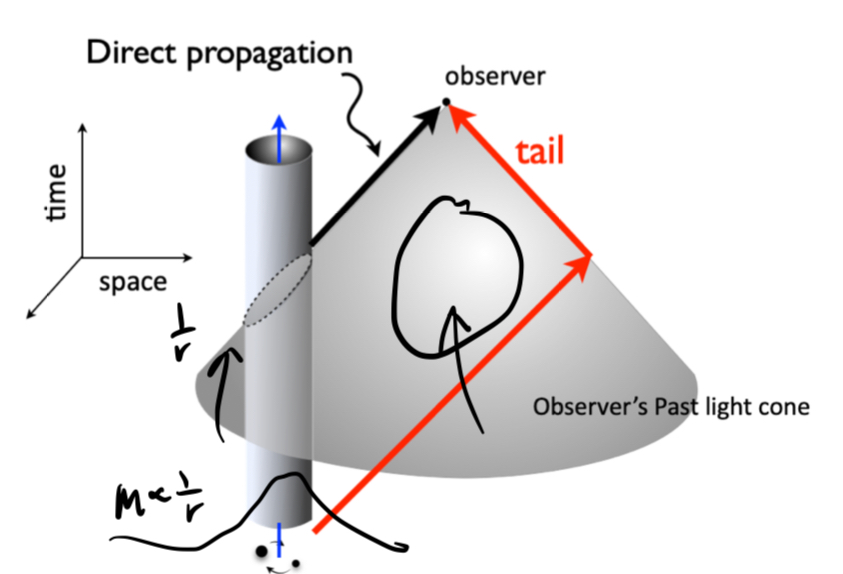
\includegraphics[scale=0.3]{Figures/tail.jpeg}
    \end{center}
    \caption{The leading-order GW tail arises from GWs scatterin g off the
      spacetime curvature due to the total mass and cause the GWs
      observed at time t to depend on the entire past history of the
      source}
    \label{fig:tail}
    \end{figure}

  \subsubsection{Memory effects}%
    \label{sub:Memory effects}
    As for the \textit{Nonlinear memory effects}, it arises from GWs that
    are sourced by previously emitted GWs. This leads to a shift in the
    oscillation amplitude and it is a non-oscillatory effect. To interpret
    this in a more \textbf{intuitive sense}, we can think of it as the
    previous GWs are not picked up by the detectors until some certain
    time (the merger GW signal is a "short" term signal).
    
    \begin{figure}[h!]
    \begin{center}
      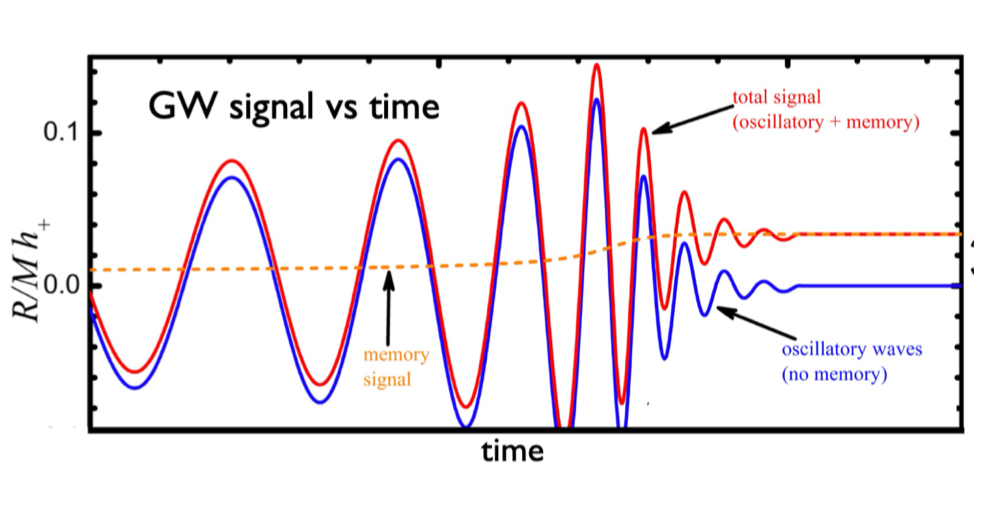
\includegraphics[scale=0.3]{Figures/memory.jpeg}
    \end{center}
    \caption{The nonlinear memory effect leads to a displacement amplitude
      before and after a burst of GWs, here a binary merger.}
    \label{fig:memory}
    \end{figure}

    \section{Application to a binary system}%
      \label{sec:Application to a binary system}
      Let us now look at some source region where the following action
      applies, \( S = S_g + S_m \), with 
      \begin{align}
        \label{action m}
        S_m &= - \sum_{\alpha = 1, 2} m_a \int \dd[]{\tau_{\alpha}} 
      \end{align}
    and the corresponding energy momentum tensor is 
    \begin{align}
      \label{energy momentum tensor for application}
      T^{\alpha\beta} &= \frac{1}{\sqrt{-g} } m
      \frac{\mathrm{d}\tau}{\mathrm{d}t}
      \frac{\mathrm{d}z^{\alpha} }{\mathrm{d}\tau}
      \frac{\mathrm{d}z^{\beta} }{\mathrm{d}\tau}
      \delta^{(3)}(\textbf{x} - \textbf{z}(t))|_{a} 
    \end{align}, where \( z^{\alpha}  \) denotes the worldline. and \(
    \frac{\mathrm{d}z^{\alpha} }{\mathrm{d}t} \) is the tangent vector to
    \( n^{\alpha}  \). 

    And now under the 3+1 decomposition, we obtain infinite self-fields
    that do not contribute to dynamics of the action, 
    \begin{align}
      \label{dynamics of action}
      S_a &= - m_a c^{2} \int \dd[]{t} \sqrt{- g_{00}^{(b)} - 2
      g_{0i}^{(b)} \frac{v_{a}^{i}}{c} - g_{ij}^{(b)}
      \frac{v_{a}^{i} v_{a}^{j}}{c^2}}  
    \end{align}, where each terms inside the square root can be
    substituted 
    perturbatively from solving EFE, also \( v_{a}^{i} \equiv
    \frac{\mathrm{d}z^{i} }{\mathrm{d}t} \). 
    After the perturbation, the action is now reduced to the so-called
    \textit{Fokker effective action} for dynamics of a.
   
   We can then move to the center of mass frame of the system and solve
   the eom up to 1 PN 
   The eom will then read 
   \begin{align}
    \label{eom with fokker effective action}
    \frac{L}{\mu} &=  \frac{v^2}{2} + \frac{GM}{r} +
     \frac{1}{c^2} \bigg\{ \frac{(1-3v)}{8}v^4 + \frac{GM}{r}
     [\frac{v}{2} \dot{r}^{2} + \frac{(3+v)}{2}v^2 ] -
     \frac{G^2 M^2}{2 r^2}  \bigg\} 
   \end{align}

   \textbf{\underline{Radiation under this action:}}\\
   Under this action, we will get the radiation as 
   \begin{align}
    \label{radiation under fokker}
    h_{ij}^{\mathrm{TT}} &= \frac{G}{c^4 R}
     \Lambda_{ijkl}^{\mathrm{TT}} [ I_{kl}^{(2)} + \frac{1}{c} N_{a} (
     \epsilon_{abck} J_{lb}^{(2)} + I_{kca}^{(2)} ) + \cdots ] 
   \end{align}, with \( I_{ij} = \mu r_{\langle ij \rangle} \) +
   \mcal{O}(\frac{1}{c^2}) 

Note that the radiation in the observer below, 
\begin{align}
  \label{observer for fokker}
  x_{\mathrm{obs}}^{j} &= R_{ij} x_{\mathrm{source}}^{j}, \hspace{0.5cm}
  R_{ij} = \begin{pmatrix} 1&0&0 \\ 
          0&\mathrm{cos}(\iota)&-\mathrm{sin}(\iota) \\ 
          0&\mathrm{sin}(\iota)&\mathrm{cos}(\iota) \end{pmatrix}
\end{align},
one can reduce the orbital parameter to simply \(
\textbf{x}_{\mathrm{source}} = r(\mathrm{cos}(\phi),
\mathrm{sin}(\phi), 0  ) \)

\subsubsection{EOM of lagrangian in circular orbits}%
  \label{sub:EOM of lagrangian in circular orbits}

  The eom of Lagrangian in circular orbits takes the following form. With
  first the three components being 
  \begin{align}
    \label{EOM of L in circular orbits}
    \ddot{r} = \dot{r} = 0, \hspace{0.5cm} \dot{\phi} = \omega,
    \hspace{0.5cm} \dot{\omega} = 0,
  \end{align}

  We can readily obtain the radial eom with the first equality 
  \begin{align}
    \label{final eom}
    0 = -\frac{GM}{r^2} + \omega^{2} + \frac{1}{c^2}[ \frac{G^2 M^2}{r^4}
    + \frac{GM \omega^2 (3 + r)}{2} + \frac{1}{2} r^2 \omega^4 (1-3r)] 
  \end{align}, where here r is gauge dependent and therefore we would like
  to express GW in terms of frequency instead, i.e. find \( r(\omega)  \). 

  To do so, we simply solve perturbatively \( r = r_0(\omega) [ 1 +
  \frac{1}{c^2} \delta r_{1}(\omega) + \cdots ] \),
  \underline{note that this is an ansatz as always.}

    We then substitute this in to eom and collect only \( 1/r \) terms 
    \begin{align}
      \label{final perturbation with eom r}
      \mcal{O}(c^0): -\frac{GM}{r_{0}^{2}} + \omega^2 &= 0 \\ 
      \mcal{O}(\frac{1}{c^2}): \frac{3GM \delta r_1}{r_{0}^{2}} +
      [\cdots]_{r_0}. 
    \end{align}
where \( r_0 = (GM)^{1/3} \omega^{-2/3}, \hspace{0.1cm} \delta r_1 =
\frac{1}{3} (GM\omega)^{2/3} (\nu-3)    \)

\subsection{Inspiral frequency correction at 1PN order}%
  \label{sub:Inspiral frequency correction at 1PN order}
  In this section, we look at the correction made to the inspiral
  system at 1PN order. 

  The first immediate change is the expression for the
  polarizations 
  \begin{align}
    \label{polarizations change at 1PN}
    h_{+} &= - \frac{G \mathcal{M}}{d c^2} \bigg(\frac{5G
    \mathcal{M}}{c^3 \tau} \bigg)^{1/4} \frac{(1 +
    \mathrm{cos}(\iota^2) )}{2} \mathrm{cos} \bigg[2 \hspace{0.1cm}
    \bigg(\frac{c^3 \tau}{5G \mathcal{M}} \bigg)^{5/8} + 2 \varphi_c
    \bigg]  \\ 
    h_{\cross} &= - \frac{G \mathcal{M}}{d c^2} \bigg(\frac{5G
    \mathcal{M}}{c^3 \tau} \bigg)^{1/4} \mathrm{cos}(\iota) \hspace{0.1cm} \mathrm{sin}
    \bigg[ 2 \hspace{0.1cm}
    \bigg(\frac{c^3 \tau}{5G \mathcal{M}} \bigg)^{5/8} + 2 \varphi_c
    \bigg].
  \end{align}

  \subsubsection{Inspiral time evaluation}%
    \label{sub:Inspiral time evaluation}
    It turns out that in the new PN order, we now have dissipative
    effect appearing in the near-zone metric at 2.5PM, which has been
    shown to be equivalent to using flux balance 
    \begin{align}
      \label{power change}
      \langle \frac{\mathrm{d}E_{\mathrm{source}}}{\mathrm{d}t} \rangle
      &= - \dot{E}_{GW} 
    \end{align}, with 

      \begin{align}
        \label{expression of E in inspiral time}
         E_{\mathrm{source}} \equiv v^{i} \frac{\partial
    \mathcal{L}}{\partial v^{i} } - \mathcal{L}
    \underbrace{=}_{\textrm{1PN}} - \frac{1}{2}\mu c^2 x[ 1  +
    (-\frac{3}{4} - \frac{\nu}{12} x) ].
      \end{align}
      Note that the term after 1 are overall negative in value, this
      means that this 1PN order correction lowers the energy of the
      source and the \textnormal{R.H.S.} of (\ref{power change})
      reads 
      \begin{align}
        \label{GW luminosity}
        \dot{E}_{\mathrm{GW}} &= \frac{32 G^{7/3} }{5 c^5}
        (\mathcal{M}\omega)^{10/3} \bigg[1 +
        \bigg(-\frac{1247}{336} - \frac{35 \nu}{12} \bigg)x
        \bigg],   
      \end{align}

      And we can then get the infamous orbital frequency via 
      \begin{align}
        \label{orbital frequency}
        \frac{\mathrm{d}\omega}{\mathrm{d}t} &= -
        \frac{\dot{E}_{GW}}{\dd[]{E}/\dd[]{\omega}} =
        \frac{96}{5 c^5} \pi^{8/3} \mathcal{M}^{5/3}
        \omega^{11/3} \bigg[1 - \bigg(\frac{743}{336} +
        \frac{11}{4} \nu \bigg) x \bigg].    
      \end{align}, where we have defined the chirp mass as \hl{$ 
      \mathcal{M}  = \mu^{3/5} M^{2/5}  $}. Also note that the
      \hl{dimensionless symmetric mass ratio} is defined as 
      \begin{align}
        \label{dimensionless symmetric mass ratio}
        \nu = \frac{\mu}{M} \in [0, 1/4]
      \end{align}, and note that it is 1/4 for equal masses and smaller
      for unequal masses. 
      

      \section{Compact objects}%
        \label{sec:Compact objects}
        
        In this section, we adopt the \textit{Geometric units}, \(
        G=c=1 \). We begin by defining a dimensionless quantity
        called compactness 
        \begin{align}
          \label{compactness}
          \frac{GM}{Rc^2} &= \frac{M}{R} 
        \end{align}. 

        \textbf{\underline{Black holes (BHs):}}
        The most renowned types of compact objects is none other than
        the BHs, which believed to obey the "no-hair" conjecture \begin{align}
          \label{no-har bro}
          Q_l + i J_l = M(i\chi M)^2
        \end{align}, with \( \chi = S/M, \hspace{0.1cm} |\chi| \leq 1
        \). Currently, we know only up to the horizon of the BHs,
        which it itself also generates deep puzzles within
        \textit{physics}, namely \textit{the information paradox.}
        In attempts to tackle this paradox, some introduce the idea
        of \textit{BH mimickers}, which are proposed solutions to
        Quantum Black Holes (QMBHs), such feats can be done by
        modifying solutions to BHs up to the horizon scale, though
        not as far as the photosphere as observations pose strong
        constraint regarding that, such modification includes
        introducing non-local quantum effects, and the idea of
        AdS/CFT from \textit{string theory}.

        \textbf{\underline{Neutron stars:}} Next up on the list we
        have neutron stars, they are the densest states of
        matter, which calls for a lot of unexplored physics, their
        usual compactness is around \( C \sim 0.2 \).  
        \begin{figure}[h!]
        \begin{center}
          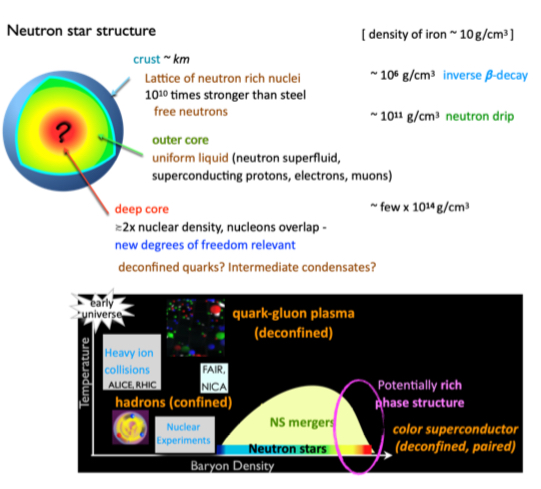
\includegraphics[scale=0.5]{Figures/neutron.jpeg}
        \end{center}
        \caption{Neutron star interiors involve a rich variety of
          physics and probe unexplored regimes of the QCD phase
          diagram.}
        \label{fig:neutron}
        \end{figure}
       
       \underline{\textbf{White dwarfs:}} These are usually around
       \( C \sim 10^{-4}  \), and they counteract gravity via
       \textit{electron degeneracy}, whatever. 

       \underline{\textbf{Dark "matter" objects:}} They are
       usually called gravitational condensates of beyond Standard
       Model (BSM). These BSM fields arise in different DM models
       and standard model extensions of particle physics.
  
      \subsection{Mathematical description of Compact Objects}%
        \label{sub:Mathematical description of Compact Objects}
        Now we commence the mathematical description of these
        objects, we first describe them via EFE and EM tensor
        conservation
        \begin{align}
          \label{EFE for compact}
          G^{\mu \nu} = 8 \pi G T^{\mu \nu}, \hspace{0.5cm}
          \nabla_{\mu} T^{\mu \nu} = 0     
        \end{align}, and for non-spinning objects, they are well
        described via Schwarzschild coordinates, which takes the form 
        \begin{align}
          \label{Schwarzschild coordinates}
          \dd[]{s}^2_0 = A(t) \dd[]{t}^{2} + B(r) \dd[]{r}^{2} +
          r^2 \dd[]{\Omega}^{2}
        \end{align}, now to solve for the whole field
        configuration, we separate to the case of interior and
        exterior of the compact object, and match the two
        solutions (\( T^{\mu}, \hspace{0.1cm} g_{\mu \nu}^{int}  \))
        with \( g_{\mu \nu}^{ext} = \textnormal{Schwarzschild
        solution for any objects} \) at \( r = R \).
        \subsubsection{Neutron stars}%
          \label{sub:Neutron stars}
          
          We can treat the interior of a neutron star as perfect
          fluid. 
          \begin{align}
            \label{neutron perfect fluid}
            T_{\mu \nu} &= (\rho + p) u_{\mu} u_{\nu} + p g_{\mu
            \nu}. 
          \end{align}, and we also need an equation of state to
          connect \( p(\rho) \), though usually this exhibits
          great uncertainties as it depends on the interior
          microphysics of the neutron star.

          \begin{figure}[h!]
          \begin{center}
            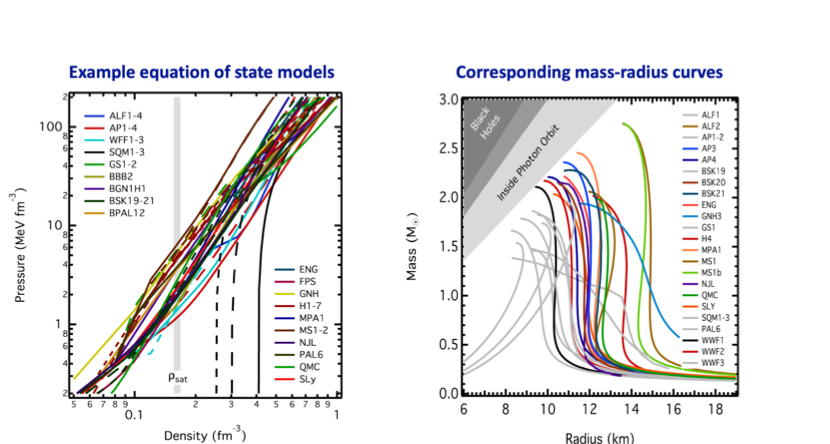
\includegraphics[scale=0.4]{Figures/interiorneutron.jpeg}
          \end{center}
          \caption{For neutron stars, the large uncertainty in the
            equation of state leads to a wide range of possible
            radii for a star with a given mass. There is a
            maximum mass beyond which the pressure can no longer
            counteract gravitational collapse, which depends on
            the equation of state. Each point on a curve
            represents a different neutron star, with decreasing
            central densities from left to right along a curve.}
          \label{fig:interiorneutron}
          \end{figure}
         \subsubsection{Binary system tidal fields}%
          \label{sub:Binary system tidal fields}
          For binary compact objects system, they are immersed in
          external tidal fields due to the companion/counterpart.
          Thus a quadrupole called tidal tensor (or
          "gravitoelectric"  STF moments) \( \epsilon_{ij} = C_{0i0j} \) is
          introduced in the object's rest frame, which is one of
          the irreducible pieces (of the Weyl tensor) with even parity, while \( C_{\mu \nu
          \alpha \beta} \) denotes the Weyl curvature tensor. The
          other irreducible pieces, which is of odd parity, is the
          "gravitomagnetic" STF tidal fields \( \mathcal{B}_{ij} \)
      \textbf{\underline{c.f.:}} In the Newtonian limit, the even
      parity piece reduces to \( l \) derivatives of the Newtonian
      gravitational potential due to the companion point mass 
      \begin{align}
        \label{newtonian tidal field}
       \epsilon_{\mathrm{Newt}}^L &= - \partial_{L}^{}
        \frac{m_2}{r}
      \end{align}

      While there is \underline{\textbf{no}} odd-parity tidal field
      in the Newtonian limit, and for non-Newtonian case, it is given by 
      \begin{align}
        \label{odd parity tidal}
        \mathcal{B}_L &= \frac{3}{2(l+1)(l-2)!} \epsilon_{\langle
        a_1 j k} C_{a_2 0; a_3\cdots a_l \rangle }^{jk}.
      \end{align}, and they can be interpreted as the relativistic
      frame-dragging fields.
      \subsection{Compact objects - Non-spinning case}%
        \label{sub:Compact objects - Non-spinning case}
       
\textbf{\underline{perturbing the metric: }}

       To solve for the tidal perturbation, we are essentially
       perturbing the metric in the form of 
       \begin{align}
        \label{tidal metric perturbation}
        \dd[]{s}^{2} &= \mathrm{d}s_{0}^{2} + \delta g_{\mu \nu}
         \mathrm{d}x^{\mu}\mathrm{d}x^{\nu},  
       \end{align}
       and similarly \( T^{\mu \nu}  = T_{0}^{\mu \nu} + \delta T^{\mu
       \nu}  \).
       Result from Regge-Wheeler in 1957 has shown that the metric
       perturbation can be splitted into 2 sectors with each of
       different parity, i.e. changing signs under the
       reflectional map \( (\theta, \phi) \mapsto (\pi - \theta, \pi +
       \phi) \). They are decomposed into 6 parts (in radial
       coordinate) as 
       \begin{align}
        \label{decomposing tidal metric perturbation}
        \delta g_{\mu \nu}^{\mathrm{even}} \mathrm{d}x^{\mu}
         \mathrm{d}x^{\nu} &=  \sum_{l,m} \bigg[- e^{-2\Phi}
         H_{0}^{lm}\mathrm{d}t^2 + 2 H_{1}^{lm} \mathrm{d}t
         \mathrm{d}r + e^{\gamma} H_{2}^{lm} \mathrm{d}r^2 + r^2
         k^{lm} \mathrm{d}\Omega^2 \bigg] Y^{lm}(\theta, \phi). 
       \end{align}, where all the \( H \) depend on \( (t, r) \) in
       general.
       
\textbf{\underline{perturbing EM tensor:}}

  Now we need to do the same for \( T^{\mu \nu}  \), though we simply need
  to decompose it in terms of the spherical harmonics via 
  \begin{align}
    \label{spherical conversion on EM tensor}
    \nabla^2 Y_{lm} &= - \frac{l(l+1)}{r^2} Y_{lm} 
  \end{align}, and then we will find that different \( (l,m) \) modes
  decouple.

  In order to get something GW-like, we need to obtain the multipoles
  of the spacetime metric, we can get the definition of the relative
  multipole moments in ACMC (asymptotic cartesian mass
  centered) coordinates.
  
  \subsection{Linear tidal response}%
    \label{sub:Linear tidal response}
    We begin by defining the linear tidal response, 
    \begin{align}
      \label{linear tidal response}
      Q_{ij} &=  - \lambda \epsilon_{ij} 
    \end{align}, where \( \lambda \) is the \hl{tidal Love number},
    that are widely studied in the literature.

    \subsection{Quadrupole effects in binaries}%
      \label{sub:Quadrupole effects in binaries}
      To obtain the quadrupole effects, we can try to solve for the
      action for a test particle 
      \begin{align}
        \label{action for tidal}
        S = m \int z \mathrm{d}t  +  \int z \mathrm{d}\tau \bigg[
        -\frac{1}{2} Q_{ij} \epsilon^{ij} +
        L^{\mathrm{internal}}(Q, \dot{Q})  \bigg]
      \end{align}, which here \( Q_{ij} \) are the small
      deviations from equilibrium.
    
    If we vary the action over \( Q_{ij} \), we get the eom 
    \begin{align}
      \label{eom for Qij}
      - \frac{1}{2} \epsilon_{ij} - 2 c_i Q_{ij} &=  0 
    \end{align}, which implies \( c_i = 1/4\lambda \)
    
    One can also define the effective/reduced worldline action, obtained
    by integrating out the quadrupole dof from the action by the results
    above, that does not depend on interal dof as 
    \begin{align}
      \label{effective reduced tidal action}
      S^{\mathrm{red}} &= m \int z \mathrm{d}\sigma +
      \frac{\lambda}{4} \int z \mathrm{d}\sigma
      \tilde{\epsilon}_{ij} \tilde{\epsilon}_{ij} + \cdots
    \end{align}, and note that all the information about the interior
    object here is encoded
    in \(  \lambda \).
\newpage
   \appendix 

   \section{BMS-group}%
    \label{sec:MBNS-group}
    There is a group of people who are working on specific type of
    GR under the Bondi-Metzner Sachs (BMS) group \( \mathfrak{B} \), which
    essentially involves extending the regular Poincare group 
    to symmetries for null-infinity, supertranslation and
    superrotational symmetry groups, please see
    \cite{ashtekar2018null} for more.  

    \newpage

\bibliographystyle{unsrt}
\bibliography{references.bib}
        
\end{document}
